%%%%%%%%%%%%%%%%%%%%%%%%%%%%%%%%%%%%%%%%%
% University Assignment Title Page 
% LaTeX Template
% Version 1.0 (27/12/12)
%
% This template has been downloaded from:
% http://www.LaTeXTemplates.com
%
% Original author:
% WikiBooks (http://en.wikibooks.org/wiki/LaTeX/Title_Creation)
%
% License:
% CC BY-NC-SA 3.0 (http://creativecommons.org/licenses/by-nc-sa/3.0/)
%
%%%%%%%%%%%%%%%%%%%%%%%%%%%%%%%%%%%%%%%%%
%\title{Title page with logo}
%----------------------------------------------------------------------------------------
%	PACKAGES AND OTHER DOCUMENT CONFIGURATIONS
%----------------------------------------------------------------------------------------

\documentclass[12pt]{article}
\usepackage[english]{babel}
\usepackage[utf8]{inputenc}
\usepackage{natbib}
\usepackage{amsmath}
\usepackage{color}
\usepackage[explicit]{titlesec}
\usepackage[hyphens,spaces,obeyspaces]{url}
\usepackage{graphicx}
\usepackage{grffile}
\usepackage{placeins}

\usepackage{pgfplots}
\usepackage{tikz,tikz-3dplot}
\usepgfplotslibrary{colormaps,fillbetween}
\pgfplotsset{compat=1.16}
\pgfplotscolormaptoshadingspec{hot}{7cm}\result
\def\tempb{\pgfdeclarehorizontalshading{tempshading}{7cm}}%
% where '\result' is inserted as last argument:
\expandafter\tempb\expandafter{\result}%
\sbox\backbox{\pgfuseshading{tempshading}}%


\begin{document}

\begin{titlepage}

\newcommand{\HRule}{\rule{\linewidth}{0.5mm}} % Defines a new command for the horizontal lines, change thickness here

\center % Center everything on the page
 
%----------------------------------------------------------------------------------------
%	HEADING SECTIONS
%----------------------------------------------------------------------------------------

\textsc{\LARGE University of St Andrews}\\[1.5cm] % Name of your university/college
\textsc{\Large CS4099}\\[0.5cm] % Major heading such as course name
\textsc{\large }\\[0.5cm] % Minor heading such as course title

%----------------------------------------------------------------------------------------
%	TITLE SECTION
%----------------------------------------------------------------------------------------

\HRule \\[0.4cm]
{ \huge \bfseries ILNP Routing for IoT}\\[0.4cm] % Title of your document
\HRule \\[1.5cm]
 
%----------------------------------------------------------------------------------------
%	AUTHOR SECTION
%----------------------------------------------------------------------------------------


\Large \emph{Author:}\\
 \textsc{Jordan Mackie}\\[1cm] % Your name
 
\Large \emph{Supervisor:}\\
 \textsc{Prof Saleem Bhatti}\\[1cm] % Your name
%----------------------------------------------------------------------------------------
%	DATE SECTION
%----------------------------------------------------------------------------------------

{\large \today}\\[2cm] % Date, change the \today to a set date if you want to be precise

%----------------------------------------------------------------------------------------
%	LOGO SECTION
%---------------------------------------------------------------------------------------


\includegraphics[width = 2.5cm]{images/standrewslogo.png}
 
%----------------------------------------------------------------------------------------

\vfill % Fill the rest of the page with whitespace

\end{titlepage}

\pagenumbering{gobble}

\section{NOTES}

\subsection{Fixing overhead}

https://ieeexplore.ieee.org/document/7993954 to fix route reply storm issue: add jitter before responding with route reply and listen for other replies

select only works in windows NOTE

Zoned Routing protocol 
Reverse Path Forwarding
Woo

\section*{Abstract}

\section*{Declaration}
I declare that the material submitted for
assessment is my own work except where credit is
explicitly given to others by citation or
acknowledgement. This work was performed during
the current academic year except where otherwise
stated.
The main text of this project report is \#TODO NN,NNN
words long, including project specification and plan.
In submitting this project report to the University of
St Andrews, I give permission for it to be made
available for use in accordance with the regulations of
the University Library. I also give permission for
the title and abstract to be published and for copies of
the report to be made and supplied at cost to any bona
fide library or research worker, and to be made
available on the World Wide Web. I retain the
copyright in this work.

\newpage

\tableofcontents

\newpage
\pagenumbering{arabic}
\setcounter{page}{1} 

\section{Introduction}

Despite the imminent exhaustion of IPv4 addresses \cite{ripe_labs}, IPv6 is still being adopted slowly \cite{google_ipv6}. Brittle solutions such as NAT are being used to expand the IPv4 address space and to avoid the transition costs involved in upgrading to IPv6. Whilst IPv6 does expand the address space greatly and introduces functionality such as multicast, the internet protocol itself suffers from many issues. 

\subsection{Issues with IP}

IP addresses are used both to identify a system and to determine its topological location. \cite{briancarpenter2014} lists several of the downsides to this overloading of IP addresses, and why the protocol was still used despite these concerns. 

The separation of concerns that should be achieved by a layered model is not possible, since the IP address is used by the each layer in some way. IP addresses can be used in the application layer, and are bound to physical network interfaces, which goes against the end-to-end argument where each layer should provide a opaque abstraction to those above it.

The issues with IP are not just semantic. Due to the overloading of the IP address and the rapid increase in internet connected devices \cite{iot_stat}, the scalability of the system is being challenged. Implementations of multipath routing with the intention of balancing load is improving network performance for the operators that use them, but with IP it places greater stress on the default-free zone (DFZ) routing information base (RIB). Multihoming is also being used to improve reliability, but with IP this requires routing entries to store multiple addresses for one host. An IAB workshop \cite{rfc4984} detailed how the DFZ RIB databases are growing in size exponentially due to the increasing number of devices and an inability to aggregate address prefixes. With IPv6 allowing for an even larger address space, this problem will only get worse. 

Due to the growing number of Internet of Things (IoT) devices, mobility is also a necessary feature for a networking protocol. Mobile IP currently requires another entity (a home agent) to track and proxy packets to the mobile host as it moves from network to network. This mobility is also problematic for IPSec, which requires that the end system addresses remain fixed.

Given the difficulty involved in simply migrating from IPv4 to IPv6, it is very doubtful that introducing an entirely different protocol for the internet would be successful. A backwards compatible solution would likely be the only solution that would be adopted within a reasonable time frame.

\subsection{ILNP}

Both multihoming and mobility are far simpler to implement and maintain if the identity and topological locator of a host are separated, and this is how the Identifier-Locator Network Protocol functions. \cite{5586444} proposes ILNPv6, which implement ILNP with the same address space as IPv6 and the same packet structure as IPv6, but with different semantics for intepreting the addresses. ILNPv6 splits the original 128-bits used for an IPv6 address into two 64-bit fields: the upper bits representing the locator and the lower 64 bits representing the identifier. The version field in the IP header is used to differentiate between ILNPv6 and IPv6 packets, and routers that don't support ILNP can interpret the packets as IP without any issue. 

The locator value identifies the subnetwork that a host belongs to, and a host can have multiple locator values, providing multihoming with smaller memory requirements for the RIB. The ID part of the address is unique to the host, and provides a fixed address which can be used at the transport layer.

Though ILNPv6 is very backwards-compatible, there are still some difficult challenges involved in its deployment. \cite{ipwithoutip} describes how the tight coupling of the C socket API and IP addresses could cause issues in some legacy applications. ILNPv6 also requires some additions to the Domain Name System (DNS) to properly support multihoming.

\subsection{Goal}

The benefits of ILNP are clear for the entire internet infrastructure. The native support for multihoming and multipath routing is especially beneficial to typically mobile internet of things (IoT) devices. This project aims to exemplify these benefits for agricultural sensor networks in particular. 

These devices are often restricted by limited battery life, memory, and computational capabilities. Most routing protocols focus on finding the shortest route between a source and destination, which often results in a small number of paths being heavily used and so some nodes are especially drained due to processing and forwarding of packets. This can result in a network partion once crucial nodes fail (due to loss of battery), rendering a section of still operational nodes useless. By reducing the networking overhead and attempting to balance traffic across several paths, the network can remain operational for longer. 

\section{Context Survey}

\subsection{Internet Routing and Addressing Architecture}

ILNP was listed alongside several other solutions to the current challenges facing the internet infrastructure in RFC6115 \cite{rfc6115}. Locator-Identifer Split Protocol (LISP) also uses locator-idnetifier semantics and has already been deployed in 60 sites over 10 countries \cite{nahla}. This ease of deployment is likely due to the fact that it requires no changes to hosts, and instead only required updates to core routers to be operational. 

Another possible alternative is Routing Architecture for the Next Generation Internet (RANGI) \cite{rangi}. RANGI again uses the identifier-locator split, but also has a cryptographic identifier which provides sender identification. 

\subsection{Energy Effecient Routing Protocols}

Wireless sensor networks (WSNs) are typically very mobile with limited memory and power, and so require optimised routing protocols. Due to the myriad of situations that IoT devices are used, there is no one-size-fits-all solution. 

\cite{hassan} classifies differeent routing protocols and provides a survey of protocols for each class. Routing protocols are either:
\begin{enumerate}
    \item \textbf{Proactive}, where each node maintains a routing table through knowledge sharing with adjacent nodes. Typically involves high overhead due to regular flooding, but performs better than reactive methods as mobility increases.
        Examples include AODV \cite{aodv} and DSR \cite{dsr}.

    \item \textbf{Reactive}, where nodes only seek out routes to remote nodes when one is required. Very little overhead in networks with low mobility, but performance degrades quickly as mobility increases.
        Examples include OLSR \cite{olsr}.
    \item \textbf{Hybrid}, where features of both proactive and reactive protocols are used.
\end{enumerate}

In typical internet infrastructure, it makes sense to use hop counts and delay as metrics for working out the 'best' routes to a destination. However, many protocol for WSNs also account for values such as remaining battery life, or how much computation the node is willing to commit to networking. 

In order to save power, MAC layer protocols will often only listen for short intervals, or rely on lower power and lower bitrate receivers to fully wake the host when communication is occuring \cite{offon}. This behaviour is one of the reasons that reactive protocols are increasingly popular for WSNs, as they don't have the high risk of signal collision that comes with frequent updates.

\subsection{IoT in Agriculture}

The sensitivity of crops to changes in climate and agricultures crucial role on national economies has naturally resulted in large amounts of research and development. \cite{agrisensor} describe how sensor technology is being used to monitor conditions in greenhouses, fields, and bodies of water. In order to make accessing this data more convenient and to help automate processes, they implemented a wireless network of enviromental sensors. These sensors communicate data to a gateway node which makes the data accessible via the cloud for visualisation and actuation. 

\cite{indoor} propose enviromental sensors but for urban environments with access to the cloud. By providing cheap montoring and actuating sensors to the general public, they hope to encourage healthier eating habits, as people would be able to grow their own vegetables effectively. 

\section{ILNP Testbed Implementation}

Due to the recency of ILNPv6, there does not currently exist software for emulating wireless ILNP networks as there is for IP, therefore a custom testbed had to be implemented. This was achieved by building an ILNP overlay network using UDP with multicast. A single UDP socket provided a communication endpoint. 

A multicast group would exist for each node ID, and so neighbours of a node would join the multicast groups of their neighbours in order to receive broadcasted packets. Figure \ref{fig:mcast} shows the ranges of each sensors radio signal as dashed lines, where each node within the range joins the multicast group.

IPv4 uses the Address Resolution Protocol (ARP) and IPv6 uses Neighbour Discovery (ND) in order to produce a mapping between IP addresses and the link layer addresses of other machines in a local network. In our overlay network, the IP addresses of the underlying network could be treated as MAC addresses. This would allow us to emulate neighbour discovery in ILNPv6, and provide unicast communication once a mapping between these virtual link layer addresses and ILNP IDs were obtained via broadcasted messages. 

\begin{figure}[!h]
	\centering
	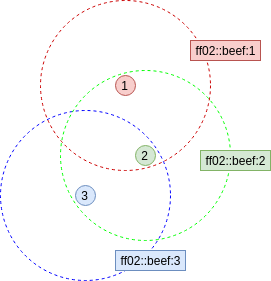
\includegraphics[width=0.5\linewidth]{images/mcast}
	\caption{Wireless broadcast emulation using multicast}
	\label{fig:mcast}
\end{figure}

\section{Protocol Design}

The protocol used is based on the Ad Hoc On-Demand Distance Vector (AODV) routing protocol, with added fields to try and account for energy usage. AODV is a reactive protocol which has three phases: discovery, maintenance, and recovery.

\subsection{Discovery}

AODV produces a list of hops that a packet can be sent over to reach a destination by flooding route request packets (RREQs). The route discovery process is summarised in figure \ref{fig:path}, where the leftmost node (1) is requesting a route to the rightmost node (4).

\begin{figure}[!h]
	\centering
	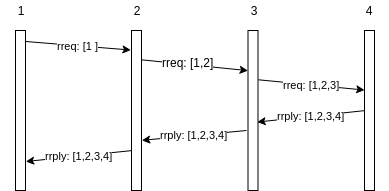
\includegraphics[width=\linewidth]{images/path}
	\caption{Route Discovery Overview}
	\label{fig:path}
\end{figure}

Figure \ref{fig:rreqflow} shows how RREQs are processed at each node. The destination node replies to all route requests for it, as this can provide multiple paths to the requesting node. Intermediate nodes however only forward requests based on whether or not they've seen them already. This can be established based on the request ID, which coupled with the source ID in the ILNP packet header can identify duplicate requests. Otherwise if this node's identifier already appears in the path so far, then it can also be discarded. These checks reduce unecessary duplication of request packets and avoid loops in the resulting paths.

When using ILNP instead of IP with AODV, packets can be routed based on the identifier alone, and this can result in multiple paths to the same node. This provides robust communication if the end destination is multihomed (i.e. has interfaces to multiple locators), with less complexity than in IP. It also makes it easier to identify disjoint paths as the node has a single name in the network, which wouldn't be the case in IP multihoming. 

\begin{figure}[!h]
	\centering
	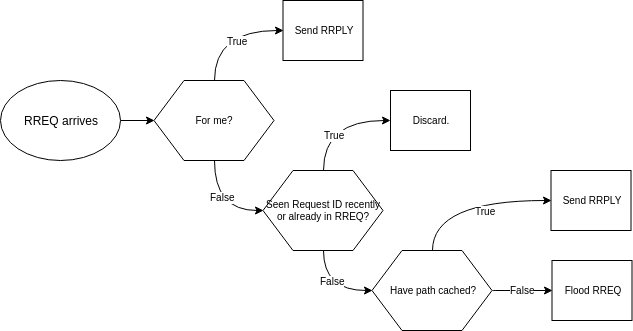
\includegraphics[width=\linewidth]{images/rreqflow}
	\caption{Route Request (RREQ) Flow}
	\label{fig:rreqflow}
\end{figure}

Once the RREQ reaches its destination, or any intermidiate node that already has a path cached to the that destination, a Route Reply (RRPLY) is generated by copying the full path from the RREQ or route cache and sending it back along the same path it arrived to the requesting node. Figure \ref{fig:rrplyflow} shows the processing that occurs at each node.

By forwarding RRPLYs along the reverse of the path that they contain, we ensure that the route hasn't broken between creation and reception of the route request. Intermediate nodes can filter erraneous route replies by only considering those where they know the next hop neighbour is still available.

This only works if we assume that all links are bidrectional which is not always the case especially in heterogenous WSNs, due to differences in transceiver ranges. 
\cite{unidirec} shows that accounting for unidirectional links in a protocol does not provide much benefit compared to the increased overhead. Also in our scenario, the nodes are likely to be homogenous and evenly spaced, so transceiver power can be assumed to be equal throughout, with no interference hot spots. 

\begin{figure}[!h]
	\centering
	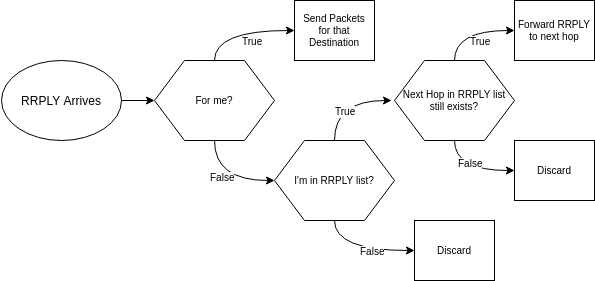
\includegraphics[width=\linewidth]{images/rrplyflow}
	\caption{Route Reply (RRPLY) Flow}
	\label{fig:rrplyflow}
\end{figure}

The structure of the route request is the same as in RFC3561 \cite{aodv}, but with an extra $\lambda$ field in the header. This value provides a metric for determining the lifespan of a route, and is calculated for an individual node using equation \ref{eq:lambda}, and visualised in Figure \ref{fig:lambda}. 

\begin{equation} \label{eq:lambda}
	\lambda = 1 -(1 - E)^2
\end{equation}

where $L$ is the \% of load the node is willing to give to networking, and $E$ is the \% battery remaining. It is based on the equation for $\lambda$ in \cite{groups}, adjusted so that $E = 0$ occurs when the battery is empty. 
The effect of decreasing $E$ was chosen so that the value of $\lambda$ would be similiar during network initialization, but to avoid network partions smaller values of $E$ would have a greater effect on $\lambda$.
Each node calculates this value before adding their ID to the path in the RREQ, and only changes the field in the packet if its calculated value is lower. 

\cite{groups} also included a load balancing factor that would account for the number of neighbours a node had, and this was considered for use in the AODV implementation. Instead of using the number of neighbours as in their link state protocol, we could use the number of nodes using a route that passed through this node. 
This value could be ascertained by counting the number of unique source IDs of packets that were forwardded. However, defining a maximum in order to normalise this factor would place restrictions on how large the network could grow. Too large and the factor has no real effect, too small and it would reduce to zero making the metric meaningless for nodes further upstream. If this number could be supplied however, it would help other nodes choose routes that aren't being used as heavily, which would be very beneficial for the lifespan of the network.

\begin{figure}[!h]
	\centering
	\begin{tikzpicture}
		\begin{axis}[set layers,view={90}{0},
			 axis lines=left,
			 grid=major,
			 no marks,
			 xmin=0, xmax=1, xlabel=$E$,
			 ymin=0, ymax=1, ylabel=$\lambda$, ylabel style={rotate=-90}
			 ]
			\addplot+[smooth,blue] {1 - (1 - x)^2}; % actual curve
			\begin{pgfonlayer}{pre main}
				\clip plot[variable=\x,samples=25,domain=0:1] (\x,{1 - (1 - \x)^2})
				|-cycle;
				\node at (0.5,0.5){\usebox\backbox};
			\end{pgfonlayer}
			% filling
		\end{axis}
	   \end{tikzpicture}\caption{Plot of Equation \ref{eq:lambda}}
	\label{fig:lambda}
\end{figure}

\subsection{Maintenance}

In order to check if neighbours are still live, \emph{HELLO} messages are exchanged at regular intervals between neighbouring nodes. These messages also provide neighbour discovery as they are limited to one hop, therefore the source ID can be mapped to the arriving IPv6 address in the emulated link layer. 

\begin{figure}[!h]
	\centering
	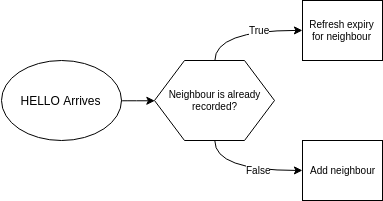
\includegraphics[width=0.6\linewidth]{images/helloflow}
	\caption{Hello Flow}
	\label{fig:helloflow}
\end{figure}

Figure \ref{fig:helloflow} shows how the \emph{HELLO} messages are processed. If a node fails to deliver a hello messages after a certain interval, then it's neighbours will begin the route recovery process.

Cached routes will also expire after some time to trigger another route request if required. This allows nodes to learn if a path is under heavy load, and ensures that a route will be corrected if for some reason the recovery process is not completed. 

\subsection{Recovery}

If the keepalive process fails for a neighbour, then a node will forward a RERR to all previous nodes in any paths it takes part in, shown in figure \ref{fig:rerrflow}.

\begin{figure}[!h]
	\centering
	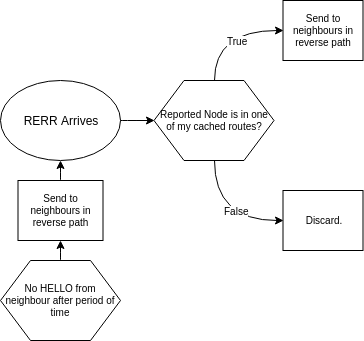
\includegraphics[width=\linewidth]{images/rerrflow}
	\caption{Route Error (RERR) Flow}
	\label{fig:rerrflow}
\end{figure}

Any packets that were sent between the failure of the link and the receiving of a route error will most likely be dropped, and future packets will be delayed as route discovery will have to take place again unless this node is aware of a disjoint path to the destination.

\FloatBarrier

\section{Software Design}

\begin{enumerate}
\item Component structure (socket interface, router/dsrservice/forwardingtable, raw sockets)
\item Runtime behaviour (packet parsing, routing, and forwarding)
\item Use figures to visualise project structure and workflow
\end{enumerate}

\section{Experiment}

\begin{enumerate}
\item Discuss aim of experiment (to measure effeciency of the used routing protocol with ILNP, and compare to IP).
\item Explain case study, with reference to source (i.e. agricultural sensor setup)
\item Use visuals to show locators to real life position and sensor radi
\item Discuss experiment configuration (how machines were chosen, results collected, battery life simulated, etc)
\item discuss choice of metrics, justifcation and how to compare results.
\end{enumerate}

\section{Results and Discussion}

\begin{enumerate}
\item Show heat map of results
\item Explain features of heat map
\item Describe the behaviour if IP was used instead through analysis
\item Discuss weaknesses with experiment
\end{enumerate}

\section{Conclusions}

Improve AODV to use locator for 'approximate' routing, then complete path once reaches locator
Mercy message to send from nodes under heavy load to try and request downstream nodes to use different paths.

\begin{enumerate}	
\item was the goal met, and if so how well?
\item future work with ILNP, possible suggestions of better alternatives to the routing protocol used.
\end{enumerate}

\section{Appendix}
\begin{enumerate}
\item Instructions on installing, and executing and using the python module, and how to configure the experiments.
\end{enumerate}

\bibliographystyle{unsrt}
\bibliography{mybib}

\end{document}
